\documentclass{lab_sheet}
\usepackage{tabularx}
\usepackage{rotating}
\usepackage[flushleft]{threeparttable}
\usepackage[hidelinks]{hyperref}
\newcommand{\figa}{
   \begin{circuitikz}[scale=0.7,american]
      \draw
      (0,0) to[R,o-o,l=$R$] (8,0)
      (6,0) to [C, *-*,l_=$C$] (6,-4)
      (0,0) to [open, v=$V_1$] (0,-4)
      (8,0) to [open, v=$V_2$] (8,-4)
      (0,-4) to [short,o-o] (8,-4)
      ;
   \end{circuitikz}
}

\newcommand{\figas}{
   \begin{circuitikz}[scale=0.7,american]
      \draw
      (0,0) to[R,o-o,l=$R$] (8,0)
      (6,0) to [C, *-*,l_=$\frac{1}{sC}$] (6,-4)
      (0,0) to [open, v=$V_1(s)$] (0,-4)
      (8,0) to [open, v=$V_2(s)$] (8,-4)
      (0,-4) to [short,o-o] (8,-4)
      ;
   \end{circuitikz}
}

\newcommand{\figb}{
   \begin{circuitikz}[scale=0.7,american]
      \draw
      (0,0) to[C,o-o,l=$C$] (8,0)
      (6,0) to [R, *-*,l_=$R$] (6,-4)
      (0,0) to [open, v=$V_1$] (0,-4)
      (8,0) to [open, v=$V_2$] (8,-4)
      (0,-4) to [short,o-o] (8,-4)
      ;
   \end{circuitikz}
}

\newcommand{\figbs}{
   \begin{circuitikz}[scale=0.7,american]
      \draw
      (0,0) to[C,o-o,l=$\frac{1}{sC}$] (8,0)
      (6,0) to [R, *-*,l_=$R$] (6,-4)
      (0,0) to [open, v=$V_1(s)$] (0,-4)
      (8,0) to [open, v=$V_2(s)$] (8,-4)
      (0,-4) to [short,o-o] (8,-4)
      ;
   \end{circuitikz}
}

\newcommand{\figc}{
   \begin{circuitikz}[scale=0.7,american]
      \draw
      (0,0) to [short,o-] (1,0) to [L,l=$L$] (3,0) to[C,l=$C$] (6,0) to[short,-o] (8,0)
      (6,0) to [R, *-*,l_=$R$] (6,-4)
      (0,0) to [open, v=$V_1$] (0,-4)
      (8,0) to [open, v=$V_2$] (8,-4)
      (0,-4) to [short,o-o] (8,-4)
      ;
   \end{circuitikz}
}

\newcommand{\figcs}{
   \begin{circuitikz}[scale=0.7,american]
      \draw
      (0,0) to [short,o-] (1,0) to [L,l=$sL$] (3,0) to[C,l=$\frac{1}{sC}$] (6,0) to[short,-o] (8,0)
      (6,0) to [R, *-*,l_=$R$] (6,-4)
      (0,0) to [open, v=$V_1(s)$] (0,-4)
      (8,0) to [open, v=$V_2(s)$] (8,-4)
      (0,-4) to [short,o-o] (8,-4)
      ;
   \end{circuitikz}
}

\newcommand{\figd}{
   \begin{circuitikz}[scale=0.7,american]
      \draw
      (0,0) to[R,o-o,l=$R$] (8,0)
      (6,0) to[L,*-,l_=$L$] (6,-2) to[C, -*,l_=$C$] (6,-4)
      (0,0) to [open, v=$V_1$] (0,-4)
      (8,0) to [open, v=$V_2$] (8,-4)
      (0,-4) to [short,o-o] (8,-4)
      ;
   \end{circuitikz}
}

\newcommand{\figds}{
   \begin{circuitikz}[scale=0.7,american]
      \draw
      (0,0) to[R,o-o,l=$R$] (8,0)
      (6,0) to[L,*-,l_=$sL$] (6,-2) to[C, -*,l_=$\frac{1}{sC}$] (6,-4)
      (0,0) to [open, v=$V_1(s)$] (0,-4)
      (8,0) to [open, v=$V_2(s)$] (8,-4)
      (0,-4) to [short,o-o] (8,-4)
      ;
   \end{circuitikz}
}

\newcommand{\fige}{
   \begin{circuitikz}[scale=0.7,american]
      \draw
      (0,0) to [short,o-] (1,0) to [R,l=$R$] (3,0) to[L,l=$L$] (6,0) to[short,-o] (8,0)
      (6,0) to [C, *-*,l_=$C$] (6,-4)
      (0,0) to [open, v=$V_1$] (0,-4)
      (8,0) to [open, v=$V_2$] (8,-4)
      (0,-4) to [short,o-o] (8,-4)
      ;
   \end{circuitikz}
}

\newcommand{\figes}{
   \begin{circuitikz}[scale=0.7,american]
      \draw
      (0,0) to [short,o-] (1,0) to [R,l=$R$] (3,0) to[L,l=$sL$] (6,0) to[short,-o] (8,0)
      (6,0) to [C, *-*,l_=$\frac{1}{sC}$] (6,-4)
      (0,0) to [open, v=$V_1(s)$] (0,-4)
      (8,0) to [open, v=$V_2(s)$] (8,-4)
      (0,-4) to [short,o-o] (8,-4)
      ;
   \end{circuitikz}
}

\newcommand{\figf}{
   \begin{circuitikz}[scale=0.7,american]
      \draw
      (0,0) to[R,o-,l=$R_1$] (4,0) to[C, l=$C_2$] (6,0) to[short,-o] (8,0)
      (4,0) to [C, *-*,l_=$C_1$] (4,-4)
      (6,0) to [R, *-*,l_=$R_2$] (6,-4)
      (0,0) to [open, v=$V_1$] (0,-4)
      (8,0) to [open, v=$V_2$] (8,-4)
      (0,-4) to [short,o-o] (8,-4)
      ;
   \end{circuitikz}
}

\newcommand{\figfs}{
   \begin{circuitikz}[scale=0.7,american]
      \draw
      (0,0) to[R,o-,i=$i_1$,l=$R_1$] (4,0) to[C, i=$i_3$, l=$\frac{1}{sC_2}$] (6,0) to[short,-o] (8,0)
      (4,0) node[label={[font=\footnotesize]above:$V_a$}] {} to [C, *-*,i=$i_2$,l_=$\frac{1}{sC_1}$] (4,-4)
      (6,0) to [R, *-*,i=$i_4$,l_=$R_2$] (6,-4)
      (0,0) to [open, v=$V_1(s)$] (0,-4)
      (8,0) to [open, v=$V_2(s)$] (8,-4)
      (0,-4) to [short,o-o] (8,-4)
      ;
   \end{circuitikz}
}

\newcommand{\proteusObservation}[5][frequency]{ 
\begin{figure}[H]
   \begin{minipage}[b]{0.60\linewidth}
     \centering
     \includegraphics[width=\linewidth]{../Figures/#2.PDF}
   \end{minipage}%
   \begin{minipage}[b]{0.40\linewidth}
     \centering
 \begin{tabular}[b]{|M{4cm}|M{1cm}|}
   \hline
   \multicolumn{2}{|c|}{Noted Values} \\
   \hline \hline
   Gain in pass band (in dB) & #3\\ \hline
   Half power #1 (in KHz) & #4\\ \hline
   Bandwidth  (in KHz)& #5\\ \hline
 \end{tabular}
 \end{minipage}
 \caption{Observation for Figure \ref{fig:#2}}
 \label{fig:prot_obs_#2}
 \end{figure}
}

\newcommand{\matlabObservation}[5][frequency]{ 
\begin{figure}[H]
   \begin{minipage}[b]{0.60\linewidth}
     \centering
     \includegraphics[width=.99\linewidth,frame]{../Figures/#2.PDF}
   \end{minipage}%
   \begin{minipage}[b]{0.40\linewidth}
     \centering
 \begin{tabular}[b]{|M{4cm}|M{1cm}|}
   \hline
   \multicolumn{2}{|c|}{Noted Values} \\
   \hline \hline
   Gain in pass band (in dB) & #3\\ \hline
   Half power #1 (in KHz) & #4\\ \hline
   Bandwidth  (in KHz) & #5\\ \hline
 \end{tabular}
 \end{minipage}
 \caption{Observation for Equation \ref{eqn:#2}}
 \label{fig:mat_obs_#2}
 \end{figure}
}
\begin{document}
\titlePage{Analysis of Filter Networks}{June 2, 2021}
\pagenumbering{roman}
\clearpage
\tableofcontents
\clearpage
\listoffigures
\clearpage
\lstlistoflistings
\clearpage
\listoftables
\clearpage
\pagenumbering{arabic}
\section{Objective}
\begin{itemize}
   \item Analyze the given filter networks.
\end{itemize}


\section{Required Tools}
\subsection{Proteus Design Suite}
Proteus Design Suite, which is a professional PCB layout, circuit design and simulation tool, will be used to
simulate the circuit for the filters to be analyzed. Proteus provides access to simulated circuit elements
and different analyzer components to visualize the response plot for the given circuits.

\subsection{MATLAB}
MATLAB is a computing platform that allows users to analyze data, develop algorithms and visualize plots, that would otherwise be a complex task.

\section{Filter Networks}
\begin{figure}[H]
   \centering
   \begin{subfigure}[b]{0.5\textwidth}
      \centering
      \figa
      \caption{}
      \label{fig:a}
   \end{subfigure}%
   \hfill
   \begin{subfigure}[b]{0.5\textwidth}
      \centering
      \figb
      \caption{}
      \label{fig:b}
   \end{subfigure}
\end{figure}
\begin{figure}[H]\ContinuedFloat
   \centering
   \begin{subfigure}[b]{0.5\textwidth}
      \centering
      \figc
      \caption{}
      \label{fig:c}
   \end{subfigure}%
   \hfill
   \begin{subfigure}[b]{0.5\textwidth}
      \centering
      \figd
      \caption{}
      \label{fig:d}
   \end{subfigure}
   \begin{subfigure}[b]{0.5\textwidth}
      \centering
      \fige
      \caption{}
      \label{fig:e}
   \end{subfigure}%
   \hfill
   \begin{subfigure}[b]{0.5\textwidth}
      \centering
      \figf
      \caption{}
      \label{fig:f}
   \end{subfigure}
   \caption{Filter networks to be analyzed}
\end{figure}

\section{Exercises}
\problem{Derive the transfer function of each of the network and determine the nature of filter network; (i.e.
whether it is lowpass, highpass, bandpass or bandstop).}
\subsubsection*{Figure \ref{fig:a}}
\begin{figure}[H]
   \centering
   \figas
\end{figure}
Using voltage divider rule,
\begin{equation}
   \begin{aligned}[b]
      V_2(s)                & =\frac{V_1(s).\frac{1}{sC}}{R+\frac{1}{sC}} \\
      \frac{V_2(s)}{V_1(s)} & =\frac{\frac{1}{sC}}{R+\frac{1}{sC}}\\
      \therefore H(s)&=\frac{1}{sRC+1}
   \end{aligned}  
   \label{eqn:matA}
\end{equation}
From the transfer function in Equation \ref{eqn:matA}, the pole is located at $-\frac{1}{RC}$ and zero is at $\infty$.
Such type of s-plane singularity position represents a \textbf{low pass} filter.
\subsubsection*{Figure \ref{fig:b}}
\begin{figure}[H]
   \centering
   \figbs
\end{figure}

Using voltage divider rule,
\begin{equation}
   \begin{aligned}[b]
      V_2(s)                & =\frac{V_1(s).R}{R+\frac{1}{sC}} \\
      \frac{V_2(s)}{V_1(s)} & =\frac{sRC}{sRC+1} \\
      \therefore H(s)&=\frac{sRC}{sRC+1}
   \end{aligned}  
   \label{eqn:matB}
\end{equation}
From the transfer function in Equation \ref{eqn:matB}, the pole is located at $-\frac{1}{RC}$ and zero is at 0. 
Such type of s-plane singularity position represents a \textbf{high pass} filter.
\subsubsection*{Figure \ref{fig:c}}
\begin{figure}[H]
   \centering
   \figcs
\end{figure}

Using voltage divider rule,
\begin{equation}
   \begin{aligned}[b]
      V_2(s)                & =\frac{V_1(s).R}{R+\frac{1}{sC}+sL} \\
      \frac{V_2(s)}{V_1(s)} & =\frac{sRC}{s^2LC+sRC+1} \\
      \therefore H(s)&=\frac{sRC}{s^2LC+sRC+1}
   \end{aligned}  
       \label{eqn:matC}
\end{equation}
The transfer function in Equation \ref{eqn:matC} is of a \textbf{band pass} filter. It can also be identified as the combination of $L$ and $C$ in the given path provides $0$ impedance at resonant frequency, which means the path is short-circuited and 
voltage across $R$ is present at output. However, at other frequencies either the capacitor or inductor causes an open-circuit resulting in a band pass nature.

\subsubsection*{Figure \ref{fig:d}}
\begin{figure}[H]
   \centering
   \figds
\end{figure}

Using voltage divider rule,
\begin{equation}
   \begin{aligned}[b]
      V_2(s)                & =\frac{V_1(s)\left(sL+\frac{1}{sC}\right)}{R+\frac{1}{sC}+sL} \\
      \frac{V_2(s)}{V_1(s)} & =\frac{s^2LC+1}{sC\left(R+\frac{1}{sC}+sL\right)} \\
      \therefore H(s)&=\frac{s^2LC+1}{s^2LC+sRC+1}
   \end{aligned}
   \label{eqn:matD}
\end{equation}
The transfer function in Equation \ref{eqn:matD} is of a \textbf{band stop} filter. It can also be identified as the combination of $L$ and $C$ across which the output is measured provides $0$ impedance at resonant frequency, which means the path is short-circuited and 
nearly $0$ voltage is present at output. However, at other frequencies either the capacitor or inductor causes an open-circuit resulting in a band stop nature.

\subsubsection*{Figure \ref{fig:e}}
\begin{figure}[H]
   \centering
   \figes
\end{figure}

Using voltage divider rule,
\begin{equation}
   \begin{aligned}[b]
      V_2(s)                & =\frac{V_1(s)\left(\frac{1}{sC}\right)}{R+\frac{1}{sC}+sL} \\
      \frac{V_2(s)}{V_1(s)} & =\frac{1}{sC\left(R+\frac{1}{sC}+sL\right)} \\
      \therefore H(s)&=\frac{1}{s^2LC+sRC+1}
   \end{aligned}
   \label{eqn:matE}
\end{equation}

The transfer function in Equation \ref{eqn:matE} is of a \textbf{low pass} filter. It can also be identified as the combination of $L$ and $R$ in the series path provides low impedance at low frequency during which the capacitor provides large impedance, which means the series path is short-circuited and 
parallel path is open-circuited. However, at higher frequencies the inductor provides larger impedance and capacitor provides lower impedance resulting in a low pass nature.

\subsubsection*{Figure \ref{fig:f}}
\begin{figure}[H]
   \centering
   \figfs
\end{figure}

To find the transfer function, using nodal analysis as,
\begin{equation}
  \begin{aligned}[b]
  \because i_3=i_4 \Rightarrow \frac{V_a(s)-V_2(s)}{\frac{1}{sC_2}}&=\frac{V_2(s)}{R_2}\\
  sR_2C_2V_a(s)&=V_2(s)(sR_2C_2+1)\\
  V_a(s)&=V_2(s)\frac{sR_2C_2+1}{sR_2C_2}
\end{aligned}
\label{eqn:matFa}
\end{equation}
\begin{equation}
   \begin{aligned}[b]
   \because i_1=i_2+i_3 \Rightarrow \frac{V_1(s)-V_a(s)}{R_1}&=\frac{V_a(s)}{\frac{1}{sC_1}}+\frac{V_a(s)-V_2(s)}{\frac{1}{sC_2}}\\
   V_1(s)-V_a(s)&=sR_1C_1V_a(s)+sR_1C_2V_a(s)-sR_1C_2V_2(s)\\
   V_1(s)&=V_a(s)(sR_1C_1+sR_1C_2+1)-sR_1C_2V_2(s)
 \end{aligned}
 \label{eqn:matFb}
 \end{equation}
 Substituting value of $V_a(s)$ from Equation \ref{eqn:matFa} into Equation \ref{eqn:matFb}, we get,
 \begin{equation}
   \begin{aligned}[b]
   V_1(s)&=V_2(s)\frac{sR_2C_2+1}{sR_2C_2}(sR_1C_1+sR_1C_2+1)-sR_1C_2V_2(s)\\
  sR_2C_2V_1(s)&=V_2(s)(s^2R_1R_2C_1C_2+s^2R_1R_2{C_2}^2+sR_2C_2+sR_1C_1+sR_1C_2+1)\\
  & \quad \quad -s^2R_1R_2{C_2}^2V_2(s)\\
  \frac{V_2(s)}{V_1(s)}&=\frac{sR_2C_2}{s^2R_1R_2C_1C_2+sR_1C_1+sR_1C_2+sR_2C_2+1}\\
  \therefore H(s)&=\frac{sR_2C_2}{s^2R_1R_2C_1C_2+s(R_1C_1+R_1C_2+R_2C_2)+1}
 \end{aligned}
 \label{eqn:matF}
 \end{equation}
The transfer function in Equation \ref{eqn:matF} is of a \textbf{band pass} filter. It can also be identified as the circuit
is a cascaded form of a RC low pass and high pass filters such that a band between their overlapping pass frequencies is created.

\problem{Plot the magnitude and phase response of each network from the derived transfer function (using
MATLAB or any tool) and note down the followings:}
\subproblem{Gain in passband}
\subproblem{Half power frequency/frequencies}
\subproblem{Bandwidth}

\matlabcode{Ashlesh_bodePlot}{Matlab function for entering transfer function and plotting bode diagram}
\matlabcode{Ashlesh_componentValues}{Matlab function that returns the component values}
\matlabcode{Ashlesh_singleScript}{Matlab script for different filter networks}

\matlabObservation{matA}{0}{1.59}{1.59}
\matlabObservation{matB}{0}{1.59}{1.59}
\matlabObservation[frequencies]{matC}{0}{1.58, 160}{158.42}
\matlabObservation[frequencies]{matD}{0}{1.57, 161}{159.43}
\matlabObservation{matE}{0}{1.6}{1.6}
\matlabObservation{matF}{-0.9}{0.180, 14.1}{13.92}

\problem{Observe the magnitude response of given filter networks by realizing the circuit using circuit
simulation tools and note down the followings:}
\subproblem{Gain in passband}
\subproblem{Half power frequency/frequencies}
\subproblem{Bandwidth}

\begin{figure}[H]
   \centering
   \begin{subfigure}[b]{0.5\textwidth}
      \centering
      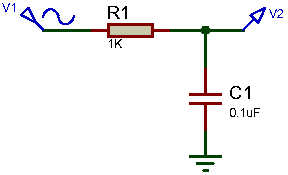
\includegraphics{../Figures/1ackt}
      \caption{}
      \label{fig:protA}
   \end{subfigure}%
   \hfill
   \begin{subfigure}[b]{0.5\textwidth}
      \centering
      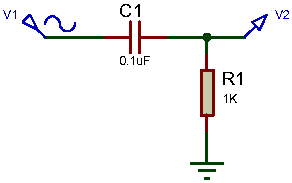
\includegraphics{../Figures/1bckt}
      \caption{}
      \label{fig:protB}
   \end{subfigure}%
   \hfill
   \begin{subfigure}[b]{0.5\textwidth}
      \centering
      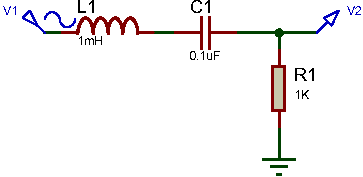
\includegraphics{../Figures/1cckt}
      \caption{}
      \label{fig:protC}
   \end{subfigure}%
   \hfill
   \begin{subfigure}[b]{0.5\textwidth}
      \centering
      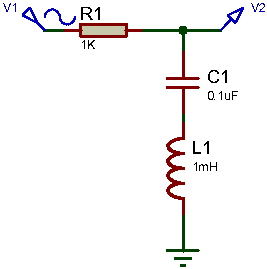
\includegraphics{../Figures/1dckt}
      \caption{}
      \label{fig:protD}
   \end{subfigure}%
   \hfill
   \begin{subfigure}[b]{0.5\textwidth}
      \centering
      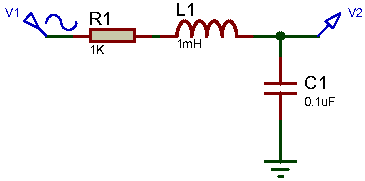
\includegraphics{../Figures/1eckt}
      \caption{}
      \label{fig:protE}
   \end{subfigure}%
   \hfill
   \begin{subfigure}[b]{0.5\textwidth}
      \centering
      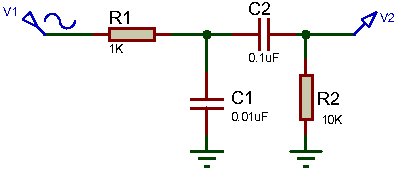
\includegraphics{../Figures/1fckt}
      \caption{}
      \label{fig:protF}
   \end{subfigure}%
   \caption{Simulated filter networks}
      \label{fig:prot}
\end{figure}
\proteusObservation{protA}{0}{1.59}{1.59}
\proteusObservation{protB}{0}{1.6}{1.6}
\proteusObservation[frequencies]{protC}{0}{1.59, 160}{158.41}
\proteusObservation[frequencies]{protD}{0}{1.57, 162}{160.43}     
\proteusObservation{protE}{0 dB}{1.6}{1.6}
\proteusObservation{protF}{-0.9 dB}{0.183, 14.1}{13.917}

\pagebreak
\subsubsection*{Compare the result obtained in Problem 2 and Problem 3.}
The observations from Figure \ref{fig:mat_obs_matA} to Figure \ref{fig:mat_obs_matF} are for the various network's response plotted using MATLAB's control system toolbox. Similarly, the observations from Figure \ref{fig:prot_obs_protA} to Figure \ref{fig:prot_obs_protF} are for the same networks simulated in Proteus. It is clear from the two sets that the variation in observation is negligible. Derived transfer functions were used to observe the response in MATLAB, which gives the theoretical values. Similarly, since Proteus is a simulated environment, practical errors aren't visible in the observed values.
\subsubsection*{Component Values  the result obtained in Problem 2 and Problem 3.}
\begin{table}[H]
   \centering
   \begin{tabular}{||M{3.5cm}||M{3cm}||}
      \hline
      \textbf{Component}&\textbf{Value}\\
      \hline
      $R$&1 K$\Omega$\\
      \hline
      $L$&1 mH\\
      \hline
      $C$&0.1 $\mu$F\\
      \hline
      $R_1$&1 K$\Omega$\\
      \hline
      $C_1$&0.01 $\mu$F\\
      \hline
      $R_2$&10 K$\Omega$\\
      \hline
      $C_2$&0.1 $\mu$F\\
      \hline
   \end{tabular}
   \caption{Original component values}
   \label{tbl:value}
\end{table}
\problem{Observe the effect in magniture response of above networks by increasing or decreasing the element values. Comment on your results for each of the given filter network.}
The values of individual components were varied by -30\%, -15\%, +15\% and +30\% as variables in MATLAB since it was easier than changing them manually in Proteus. The change in parameters such as Gain in pass band, Half power frequency/frequencies and Bandwidth due to the variation in component values were observed.
\begin{sidewaystable}
   \begin{threeparttable}
      \scriptsize
   \begin{tabularx}{\textwidth}{@{}||>{\centering\arraybackslash}X||>{\centering\arraybackslash}X||*{5}{c|c|c||}@{}}
      \cline{1-17}
      \parbox[t]{2mm}{\multirow{3}{*}{\rotatebox[origin=c]{90}{Figure}}}&\parbox[t]{2mm}{\multirow{3}{*}{\rotatebox[origin=c]{90}{Component}}}  & \multicolumn{15}{c||}{\% change in component values} \\
       \cline{3-17}
   &   &\multicolumn{3}{c||}{$-30$}&\multicolumn{3}{c||}{$-15$}&\multicolumn{3}{c||}{$0$}&\multicolumn{3}{c||}{$+15$}&\multicolumn{3}{c||}{$+30$}\\
   \cline{3-17}
   &   & G & $f$ & $\omega$ & G & $f$ & $\omega$ & G & $f$ & $\omega$ & G & $f$ & $\omega$ & G & $f$ & $\omega$ \\
   \cline{1-17}
   \multirow{2}{*}{\ref{fig:a}}&$R$&0&2.27&2.27&0&1.87&1.87&\multirow{2}{*}{0}&\multirow{2}{*}{1.59}&\multirow{2}{*}{1.59}&0&1.38&1.38&0&1.22&1.22\\
   \cline{2-8}\cline{12-17}
   &$C$&0&2.27&2.27&0&1.87&1.87&&&&0&1.38&1.38&0&1.22&1.22\\
   \cline{1-17}
   \multirow{2}{*}{\ref{fig:b}}&$R$&0&2.28&2.28&0&1.88&1.88&\multirow{2}{*}{0}&\multirow{2}{*}{1.59}&\multirow{2}{*}{1.59}&0&1.39&1.39&0&1.23&1.23\\
   \cline{2-8}\cline{12-17}
   &$C$&0&2.28&2.28&0&1.88&1.88&&&&0&1.39&1.39&0&1.23&1.23\\
   \cline{1-17}
   \multirow{3}{*}{\ref{fig:c}}&$R$&0&2.24, 113&110.76&0&1.86, 137&135.14&\multirow{3}{*}{0}&\multirow{3}{*}{1.58, 160}&\multirow{3}{*}{158.42}&0&1.38, 184&182.62&0&1.22, 207&205.78\\
   \cline{2-8}\cline{12-17}
   &$L$&0&1.59, 228&226.43&0&1.59, 188&186.41&&&&0&1.58, 140&138.42&0&1.58, 124&122.42\\
   \cline{2-8}\cline{12-17}
   &$C$&0&2.25, 160&157.75&0&1.86, 160&158.14&&&&0&1.38, 160&158.62&0&1.22, 160&158.78\\
   \cline{1-17}
   \multirow{3}{*}{\ref{fig:d}}&$R$&0&2.22, 114&111.78&0&1.84, 138&136.16&\multirow{3}{*}{0}&\multirow{3}{*}{1.57, 161}&\multirow{3}{*}{159.43}&0&1.37, 185&183.63&0&1.21, 209&207.79\\
   \cline{2-8}\cline{12-17}
   &$L$&0&1.57, 230&228.43&0&1.57, 189&187.43&&&&0&1.57, 140&138.43&0&1.56, 125&123.44\\
   \cline{2-8}\cline{12-17}
   &$C$&0&2.23, 161&158.77&0&1.85, 161&159.15&&&&0&1.37, 161&159.63&0&1.21, 161&159.79\\
   \cline{1-17}
   \multirow{3}{*}{\ref{fig:e}}&$R$&0&2.31&2.31&0&1.89&1.89&\multirow{3}{*}{0}&\multirow{3}{*}{1.6}&\multirow{3}{*}{1.6}&0&1.39&1.39&0&1.23&1.23\\
   \cline{2-8}\cline{12-17}
   &$L$&0&1.6&1.6&0&1.6&1.6&&&&0&1.6&1.6&0&1.6&1.6\\
   \cline{2-8}\cline{12-17}
   &$C$&0&2.3&2.3&0&1.89&1.89&&&&0&1.39&1.39&0&1.23&1.23\\
   \cline{1-17}
   \multirow{4}{*}{\ref{fig:f}}&$R_1$&-0.6&0.173, 20.9&20.727&-0.7&0.177, 16.9&16.723&\multirow{4}{*}{-0.9}&\multirow{4}{*}{0.18, 14.1}&\multirow{4}{*}{13.92}&-1.05&0.184, 12&11.816&-1.2&0.189, 10.3&10.111\\
   \cline{2-8}\cline{12-17}
   &$C_1$&-0.9&0.18, 20.1&19.92&-0.9&0.18, 16.5&16.32&&&&-0.9&0.18, 12.2&12.02&-0.9&0.18, 10.8&10.62\\
   \cline{2-8}\cline{12-17}
   &$R_2$&-1.3&0.276, 13.1&12.824&-1.06&0.217, 13.7&13.483&&&&-0.8&0.154, 14.3&14.146&-0.7&0.134, 14.5&14.366\\
   \cline{2-8}\cline{12-17}
   &$C_2$&-0.9&0.258, 14&13.742&-0.9&0.212, 14&13.788&&&&-0.9&0.157, 14&13.843&-0.9&0.139, 14&13.861\\
   \cline{1-17}
\end{tabularx}   
 \begin{tablenotes}
    \item[1] G : Gain in pass band (in dB)
    \item[2] $f$ : Half power frequency (in KHz)
    \item[3] $\omega$ : Bandwidth (in KHz)
   \end{tablenotes}
\end{threeparttable}
  \caption{Observation for increase and decrease in component values}
  \label{tbl:obs}
\end{sidewaystable}
\newpage
Table \ref{tbl:obs} shows a detailed observation for the parameters variation with change in component values. For low pass filter and high pass filter given in Figure \ref{fig:a} and Figure \ref{fig:b} respectively, the variation in either $R$ or $C$ showed similar behavior variation. For decrease in the value, the half power frequency and bandwidth increased, whereas with increase in the value, the half power frequency and bandwidth decreased.\\
For band pass filter and band stop filter given in Figure \ref{fig:c} and Figure \ref{fig:d} respectively, the decrease in value of $R$ increased the lower half power frequency whereas decreased the upper half power frequency, leading to a decrease in bandwidth. On the contrary, increase in the value of $R$ decreased the lower limit of the band whereas increased the upper limit, leading to an increase in bandwidth. For variation in $L$, negligible change was seen in the lower limit, whereas inverse change was observed for the upper limit, leading to an over all inverse relation for the bandwidth. For variation in $C$, negligible variation was seen in the upper limit, whereas inverse relation with the lower limit was observed. This lead to an overall direct relationship with the bandwidth change for variation in $C$. 
\\For low pass filter given in Figure \ref{fig:e}, variation in $R$ or $C$ had an identical inverse effect on the half power frequency and bandwidth. However, for the variation in $L$, no change was observed for any parameters.\\
No change in gain in pass band was observed yet.\\
For band pass filter given in Figure \ref{fig:f}, the decrease in $R_1$ decreased the lower limit of the band whereas the upper frequency increased leading to an increase in bandwidth. Similarly the gain in bass band also increased. On the other hand, increase in the value of $R_1$ increased the lower frequency and decreased the upper limit of the band which led to a decrease in bandwidth. The gain in pass band decreased during this variation. For variation in $C_1$, the lower frequency of the band remained unchanged, whereas the upper limit showed an inverse relation leading to an overall inverse relation with bandwidth. The gain in pass band remained unchanged. For decrease in $R_2$, the lower limit of the band increased and the upper frequency decreased which meant the bandwidth decreased. The gain in pass band decreased. Likewise, for the increase in the value of $R_2$, the lower frequency decreased and upper frequency increased leading to an increase in bandwidth. The gain in pass band increased during this variation. For variation in $C_2$, the upper frequency of the band remained somewhat unchanged, whereas the lower limit showed an inverse relation. The relation with bandwidth was somewhat uneven as indicated by the tabulated value. The gain in pass band remained unchanged.
\section{Conclusion}
The lab experiment for Analysis of Filter Networks concluded following the realization of the objectives. The analysis of filter networks based on their network elements, transfer functions, simulated plot allowed the visualization of the responses and determination of the different parameters.
\end{document}